\documentclass{scrreprt}

\usepackage{aligned-overset}
\usepackage{amsmath}
\usepackage{amssymb}
\usepackage{bm}
\usepackage[shortlabels]{enumitem}
\usepackage{hyperref}
\usepackage[utf8]{inputenc}
\usepackage{multicol}
\usepackage{mathtools}
\usepackage{physics}
\usepackage{pdflscape}
\usepackage{tabularx}
\usepackage{titling}
\usepackage{fancyhdr}
\usepackage{xfrac}
\usepackage[dvipsnames]{xcolor}
\usepackage{pgfplots}

\pgfplotsset{compat = newest}
\usetikzlibrary{intersections}
\usetikzlibrary{patterns}
\usepgfplotslibrary{fillbetween}

\author{Karsten Lehmann (Übungsgruppe 1)\\Mat. Nr 4935758}
\date{WiSe 2021/2022}
\title{Hausaufgaben Blatt 13\\Analysis - Grundlegende Konzepte}

\setlength{\headheight}{26pt}
\pagestyle{fancy}
\fancyhf{}
\lhead{\thetitle}
\rhead{\theauthor}
\lfoot{\thedate}
\rfoot{Seite \thepage}

\begin{document}
\paragraph{69. Im Folgenden sollen Sie ein Additionstheorem für die Tangensfunktion beweisen}
\begin{enumerate}[(a)]
\item Seien $x, y \in \mathbb{R} \setminus \qty{k\pi + \frac{\pi}{2}
    \,\middle|\, k \in \mathbb{Z}}$.
  Bestimmen Sie $y$ in Abhängigkeit von $x$, sodass die Gleichung
  \[
    \tan\qty\big(x)\tan\qty\big(y) = 1
  \]
  gilt.
  Welche Bedingung erfüllt $x + y$.

  \subparagraph{Lsg.} Es ist $\tan x = \frac{\sin x}{\cos x}$ für
  $x \in \mathbb{R} \setminus \qty{\frac{\pi}{2} + k\pi
    \,\middle|\, k \in \mathbb{Z}}$ und
  $\cos\qty\big(x + y) = \cos x \cos y - \sin x \sin y$.
  \begin{flalign*}
    \tan\qty\big(x)\tan\qty\big(y) &= 1 \\
    \frac{\sin x}{\cos x} \cdot \frac{\sin y}{\cos y} &= 1
    &&{\Big |} \cdot \frac{\cos y}{\sin y} \\
    \frac{\sin x}{\cos x} &= \frac{\cos y}{\sin y} \\
    \sin x \sin y &= \cos x \cos y \\
    0 &= \cos x \cos y - \sin x \sin y \\
    0 &= \cos\qty\big(x + y) &\overset{\text{Satz 13.20}}&\iff \\
    x + y &= \frac{\pi}{2} + k\pi, k \in \mathbb{Z}
  \end{flalign*}

  $\Rightarrow$ \underline{$y = \frac{\pi}{2} + k\pi - x$, $k \in \mathbb{Z}$}.

\item Es seien $x, y \in \mathbb{R} \setminus \qty{k\pi + \frac{\pi}{2}
    \,\middle|\, k \in Z}$.
  Beweisen Sie, dass
  \[
    \tan\qty\big(x + y) = \frac{\tan\qty\big(x) + \tan\qty\big(y)}
    {1 - \tan\qty\big(x)\tan\qty\big(y)}
  \]

  \subparagraph{Lsg.}
  \begin{flalign*}
    \frac{\sin\qty\big(x + y)}{\cos\qty\big(x + y)}
    &= \frac{\frac{
        \sin x}{\cos x} + \frac{\sin y}{\cos y}
    }{
      1 - \frac{\sin x}{\cos x}\frac{\sin y}{\cos y}
    } && {\Big |}\, \cdot \cos x \cos y\\
    &= \frac{\sin x \cos y + \sin y \cos x}{\cos x \cos y - \sin x \sin y} \\
    \overset{\text{Satz 13.15 (4)}}&=
    \frac{\sin\qty\big(x + y)}{\cos\qty\big(x + y)}
  \end{flalign*}
\end{enumerate}

\newpage
\paragraph{70. In dieser Aufgabe sollen Sie die Anwendung der Polarkoordinaten
  komplexer Zahlen üben.}
\begin{enumerate}[(a)]
\item Geben Sie mit Hilfe der Exponentialdarstellung einer Zahl
  $z \in \mathbb{C}$ eine geometrische Interpretation der Multiplikation
  in $\mathbb{C}$ in der komplexen Zahlebene.

  \subparagraph{Lsg.} Seien $z_1, z_2 \in \mathbb{C}$ und
  $\xi_1, \xi_2 \in \big[0, 2\pi\big)$ so gewählt, dass
  $z_1 = \abs{z_1} \cdot e^{\xi_1 \cdot i}$ und
  $z_2 = \abs{z_2} \cdot e^{\xi_2 \cdot i}$.

  Nun ist $z_1 \cdot z_2 = \abs{z_1} e^{i \xi_1} \cdot \abs{z_2} e^{i \xi_2}
  = \abs{z_1 z_2} e^{i\qty\big(\xi_1 + \xi_2)}$.

  \begin{tikzpicture}[scale=1.5]
    \begin{axis}[
      axis x line=center,
      axis y line=center,
      grid=both,
      xlabel={Re},
      xmin=-2.1,
      xmax=2.1,
      xticklabels={,,},
      ylabel={Im},
      ymin=-2.1,
      ymax=2.1,
      yticklabels={,,},
    ]
      \node[circle, fill, label=right:{$z_1$}, inner sep=2pt] at (0.5,1) {};
      \node at (0.2, 0.1) {\tiny $\xi_1$};
      \node[black!70!green, circle, fill, label=above:{$z_2$}, inner sep=2pt] at (-0.4,0.4) {};
      \node[black!70!green] at (-0.07, 0.2) {\tiny $\xi_2$};
      \node[black!50!red, circle, fill, label=below:{$z_1 \cdot z_2$}, inner sep=2pt] at (-1.74,-0.57) {};
      \node[black!50!red] at (-1.3, 0.5) {\tiny $\xi_1 + \xi_2$};

      \draw (0,0) -- (0.5,1) node[right, pos=.5] {\tiny $\abs{z_1}$};
      \draw (0.3,0) arc (0:64:0.3);

      \draw[black!70!green] (0,0) -- (-0.4,0.4) node[below left = -3pt, black!70!green, pos=.5] {\tiny $\abs{z_2}$};
      \draw[black!70!green] (0.35,0) arc (0:135:0.35);

      \draw[black!50!red] (0,0) -- (-1.74,-0.57) node[below=4pt, black!50!red, pos=.5] {\small $\abs{z_1 + z_2}$};
      \draw[black!50!red] (1,0) arc (0:198:1);
    \end{axis}
  \end{tikzpicture}

\item Bestimmen Sie Real- und Imaginärteil der komplexen Zahl
  $\qty\big(\sqrt{3} + i)^{2022}$.

  \subparagraph{Lsg.} Es ist $\abs{\sqrt{3} + i} = \sqrt{\sqrt{3}^2 + 1^2}
  = \sqrt{4} = 2$.

  Nun wird ein $\xi$ mit
  $\sqrt{3} + i = 2 \cdot \qty\Big(\frac{\sqrt{3}}{2} + \frac{i}{2})
  = 2 \cdot \qty\big(\cos \xi + i \sin \xi)$.
  Aus der Tabelle zu Sinus und Cosinus im Skript (nach Satz 13.20) folgt
  $\xi = \frac{\pi}{6}$.

  $\Rightarrow \sqrt{3} + i = 2 e^{i \frac{\pi}{6}}$
  $\Rightarrow \qty\big(\sqrt{3} + i)^{2022}
  = 2^{2022} e^{i \cdot 2022 \cdot \frac{\pi}{6}}
  \overset{\text{Satz 13.19 (1)}}= 2^{2022} e^{i \pi}$

  \begin{tikzpicture}[scale=1]
    \begin{axis}[
      axis x line=center,
      axis y line=center,
      grid=both,
      xlabel={Re},
      xmin=-1.1,
      xmax=1.1,
      xticklabels={,,},
      ylabel={Im},
      ymin=-1.1,
      ymax=1.1,
      yticklabels={,,},
    ]
      \node[circle, fill, label=below right:{$\qty\big(\sqrt{3} + i)^{2022}$}, inner sep=2pt] at (-1,0) {};
      \node at (-0.3, 0.2) {\small $\pi$};
      \draw (0.5,0) arc (0:180:0.5);
    \end{axis}
  \end{tikzpicture}

  $\Rightarrow \Re \qty\big(\sqrt{3} + i)^{2022} = - 2^{2022}$

  $\Rightarrow \Im \qty\big(\sqrt{3} + i)^{2022} = 0$

\item Bestimmen Sie alle komplexen 3-ten Wurzeln von $-8i$.

  \subparagraph{Lsg.} Es ist $\abs{-8i} = 8$.
  Nun ist ein $\xi$ gesucht mit $-8i = 8 \cdot \qty\big(\cos \xi + i \sin \xi)$.
  Aus der Tabelle zu Sinus und Cosinus im Skript (nach Satz 13.20) folgt
  $\xi = -\frac{\pi}{2}$.

  Aus Satz 13.21 (3) der Vorlesung (``$w^n = z \iff
  w \in \qty{\sqrt[n]{\abs{z}}e^i\qty(\frac{\xi}{n} + \frac{2k\pi}{n})}$'')
  folgt
  \begin{enumerate}[label={$w_{\arabic*} =$}]
  \item $2 \cdot e^{i -\frac{\pi}{6} + \frac{2 \cdot 1 \pi}{3}} = 2 \cdot e^{i \frac{3\pi}{6}} = 2 \cdot e^{i \frac{\pi}{2}}$ 
  \item $2 \cdot e^{i -\frac{\pi}{6} + \frac{2 \cdot 2 \pi}{3}} = 2 \cdot e^{i \frac{7\pi}{6}}$
  \item $2 \cdot e^{i -\frac{\pi}{6} + \frac{2 \cdot 3 \pi}{3}} = 2 \cdot e^{i \frac{11\pi}{6}}$
  \end{enumerate}

\item Es seien $n \in \mathbb{N}$ und $\varphi \in \mathbb{R}$.
  Beweisen Sie die Formel
  \[
    \qty\big(\cos \varphi + i \sin \varphi)^n = \cos\qty\big(n\varphi) + i \sin\qty\big(n\varphi)
  \]

  \subparagraph{Lsg.} Nach Satz 13.21 (2) der Vorlesung gilt für
  $z \in \mathbb{C}$ und $\xi \in \big[0, 2\pi \big)$, dass
  $\abs{z} \cdot e^{i\xi} = \abs{z}\qty\big{\cos\xi + i\sin\xi}$.
  Es folgt $e^{i\xi} = \cos\xi + i\sin\xi$.

  $\Rightarrow \qty\big(\cos \varphi + i \sin \varphi)^n =
  e^{i\varphi} \cdot e^{i\varphi} \cdot \ldots \cdot e^{i\varphi}
  = e^{in\varphi} = \cos\qty\big(n\varphi) + i\sin\qty\big(n\varphi)$
\end{enumerate}

\newpage
\paragraph{71. Beweisen Sie die folgenden Gleichungen und Ungleichungen:}

\begin{enumerate}[(a)]
\item Es sei $z \in \mathbb{C}$.
  Dann gilt
  \[
    \cosh^2\qty\big(z) - \sinh^2\qty\big(z) = 1
  \]

  \subparagraph{Lsg.} Es ist $\sinh z = \frac{e^z - e^{-z}}{2}$ und
  $\cosh z = \frac{e^z + e^{-z}}{2}$
  \begin{flalign*}
    \cosh^2\qty\big(z) - \sinh^2\qty\big(z)
    &= \qty(\frac{e^z + e^{-z}}{2})^2 - \qty(\frac{e^z - e^{-z}}{2})^2 \\
    &= \frac{e^{2z} + 2 \cdot e^{z - z} + e^{-2z}}{4} - \frac{e^{2z} - 2e^{z - z} + e^{-2z}}{4} \\
    &= \frac{4e^0}{4} = 1
  \end{flalign*}

\item Es seien $z, w \in \mathbb{C}$.
  Dann gilt
  \[
    \sinh\qty\big(z + w) = \sinh\qty\big(z)\cosh\qty\big(w) + \sinh\qty\big(w)\cosh\qty\big(z)
  \]

  \subparagraph{Lsg.} Nach Satz 13.22 (1) der Vorlesung ist
  $\sinh z = -i\sin\qty\big(iz)$ und $\cosh\qty\big(z) = \cos\qty\big(iz)$.

  Somit ist
  \begin{flalign*}
    \sinh\qty\big(z + w) &= -i \sin\qty\big(-iz - iw) \\
    \overset{\text{13.15 (4)}}&= -i \qty\Big(
      \sin\qty\big(-iz)\cos\qty\big(-iw) + \sin\qty\big(-iw)\cos\qty\big(-iz)
    ) \\
    &= -i \sin\qty\big(-iz)\cos\qty\big(-iw) - i \sin\qty\big(-iw)\cos\qty\big(-iz) \\
    \overset{\text{Satz 13.22 (1)}}&= \sinh\qty\big(z)\cosh\qty\big(w) + \sinh\qty\big(w)\cosh\qty\big(z)
  \end{flalign*}

\item Es sei $x \in \mathbb{R}$.
  Dann gilt
  \[
    \sinh\qty\big(x) < \frac{e^x}{2} < \cosh\qty\big(x)
  \]

  \subparagraph{Lsg.} Es ist $\sinh z = \frac{e^z - e^{-z}}{2}$ und
  $\cosh z = \frac{e^z + e^{-z}}{2}$.
  Weiterhin wurde in Aufgabe 64 (c) bereits gezeigt, dass $e$ eine positive
  reelle Zahl ist.
  Nach Satz 5.20 (2) der Vorlesung folgt $0 < e^r$ für jedes beliebige
  $r \in \mathbb{R}$ (auch $r = -x$).
  Aus Satz 5.4 (3) der Vorlesung folgt $-e^{-x} < 0$.

  Kombiniert man diese beiden Folgerungen kommt man mittels äquivalenter
  Umformungen auf den gesuchten Ausdruck:
  \begin{flalign*}
    -e^{-x} < 0 &< e^{-x} && {\Big |} + e^{x} && \\
    e^x - e^{-x} < e^x &< e^x + e^{-x} && {\Big |} :2 \\
    \frac{e^x - e^{-x}}{2} < \frac{e^x}{2} &< \frac{e^x + e^{-x}}{2}
  \end{flalign*}
\end{enumerate}

\end{document}
